\chapter{Memory Allocators}

\epigraph{Memory memory everywhere but not an allocation to be made}{A really fragmented heap}

\section{Introduction}

Memory allocation is very important!
Allocating and deallocating heap memory is one of the most common operations in any application.
The heap at the system level is contiguous series of addresses that the program can expand or contract and use as its own accord \cite{mallocinternals}.
In POSIX, this is called the system break.
We use \keyword{sbrk} to move the system break.
Most programs don't interact directly with this call, they use a memory allocation system around it to handle chunking up and keeping track of which memory is allocated and which is freed.

We will mainly be looking into simple allocators.
Just know that there are other ways of dividing up memory like with \keyword{mmap} or other allocation schemes and methods like \keyword{jemalloc}.

\section{C Memory Allocation API}

\begin{itemize}

\item \keyword{malloc(size\_t bytes)} is a C library call and is used to reserve a contiguous block of memory that may be uninitialized \cite[P. 348]{jones2010wg14}.
Unlike stack memory, the memory remains allocated until \keyword{free} is called with the same pointer.
If \keyword{malloc} can either return a pointer to at least that much free space requested or \keyword{NULL}.
That means that malloc can return NULL even if there is some spaces.
Robust programs should check the return value.
If your code assumes \keyword{malloc} succeeds, and it does not, then your program will likely crash (segfault) when it tries to write to address 0.
Also, malloc may not zero out memory because of performance -- check your code to make sure that you are not using uninitialized values.

\item \keyword{realloc(void *space, size\_t bytes)} allows you to resize an existing memory allocation that was previously allocated on the heap (via malloc, calloc, or realloc) \cite[P. 349]{jones2010wg14}.
The most common use of realloc is to resize memory used to hold an array of values.
There are two gotchas with realloc.
One, a new pointer may be returned.
Two, it can fail.
A naive but readable version of realloc is suggested below with sample usage.

\begin{lstlisting}[language=C]
void * realloc(void * ptr, size_t newsize) {
  // Simple implementation always reserves more memory
  // and has no error checking
  void *result = malloc(newsize);
  size_t oldsize =  ... //(depends on allocator's internal data structure)
  if (ptr) memcpy(result, ptr, newsize < oldsize ? newsize : oldsize);
  free(ptr);
  return result;
}

int main() {
  // 1
  int *array = malloc(sizeof(int) * 2);
  array[0] = 10; array[1] = 20;
  // Oops need a bigger array - so use realloc..
  array = realloc(array, 3 * sizeof(int));
  array[2] = 30;

}
\end{lstlisting}

The above code is not robust.
If \keyword{realloc} fails then the array is a memory leak.
Robust code checks for the return value and only reassigns the original pointer if not null.

\begin{lstlisting}[language=C]
int main() {
  // 1
  int *array = malloc(sizeof(int) * 2);
  array[0] = 10; array[1] = 20;
  void *tmp = realloc(array, 3 * sizeof(int));
  if (tmp == NULL) {
    // Nothing I can do here
  } else if (tmp == array) {
    // realloc returned same space
    array[2] = 30;
  } else {
    // realloc returned different space
    array = tmp;
    array[2] = 30;
  }

}
\end{lstlisting}

\item \keyword{calloc(size\_t nmemb, size\_t size)} initializes memory contents to zero and also takes two arguments: the number of items and the size in bytes of each item.
An advanced discussion of these limitations is \href{http://locklessinc.com/articles/calloc/}{in this article}.
Programmers often use \keyword{calloc} rather than explicitly calling \keyword{memset} after \keyword{malloc}, to set the memory contents to zero because certain performance considerations are taken into account.
Note \keyword{calloc(x,y)} is identical to \keyword{calloc(y,x)}, but you should follow the conventions of the manual.
A naive implementation of calloc is below.

\begin{lstlisting}[language=C]
void *calloc(size_t n, size_t size) {
  size_t total = n * size; // Does not check for overflow!
  void *result = malloc(total);

  if (!result) return NULL;

  // If we're using new memory pages
  // just allocated from the system by calling sbrk
  // then they will be zero so zero-ing out is unnecessary,
  // We will be non-robust and memset either way.
  return memset(result, 0, total);
}
\end{lstlisting}

\item \keyword{free} takes a pointer to the start of a piece of memory and makes it available for use in subsequent calls to the other allocation functions.
This is important because we don't want every process in our address space to take an enormous amount of memory.
Once we are done using memory, we stop using it with free.
A simple usage is below.

\begin{lstlisting}[language=C]
int *ptr = malloc(sizeof(*ptr));
do_something(ptr);
free(ptr);
\end{lstlisting}

If you use a piece of memory after it is freed - that is undefined behavior.

\end{itemize}

\subsection{Heaps and sbrk}

The heap is part of the process memory, and it does not have a fixed size.
Heap memory allocation is performed by the C library when you call \keyword{malloc} (\keyword{calloc}, \keyword{realloc}) and \keyword{free}.
By calling \keyword{sbrk} the C library can increase the size of the heap as your program demands more heap memory.
As the heap and stack need to grow, we put them at opposite ends of the address space.
Stacks don't grow like a heap, new parts of the stack are allocated for new threads.
So for typical architectures the heap will grow upwards and the stack grows downwards.

Nowadays, Modern operating system memory allocators no longer need \keyword{sbrk} - instead they can request independent regions of virtual memory and maintain multiple memory regions.
For example, gibibyte requests may be placed in a different memory region than small allocation requests.
However this detail is an unwanted complexity.

Programs don't need to call \keyword{brk} or \keyword{sbrk} typically, though calling \keyword{sbrk(0)} can be interesting because it tells you where your heap currently ends.
Instead programs use \keyword{malloc},\keyword{calloc},\keyword{realloc} and \keyword{free} which are part of the C library.
The internal implementation of these functions may call \keyword{sbrk} when additional heap memory is required.

\begin{lstlisting}[language=C]
void *top_of_heap = sbrk(0);
malloc(16384);
void *top_of_heap2 = sbrk(0);
printf("The top of heap went from %p to %p \n", top_of_heap, top_of_heap2);
// Example output: The top of heap went from 0x4000 to 0xa000
\end{lstlisting}

An important fact we just glossed over earlier is memory that was newly obtained by the operating system must be zeroed out.
If the operating system did not zero out contents of physical RAM, it might be possible for one process to learn about the memory of another process that had previously used the memory.
This would be a security leak.
Unfortunately this means that for \keyword{malloc} requests before any memory has been freed is \emph{often} zero.
This is unfortunate because many programmers mistaken write C programs that assume allocated memory will \emph{always} be zero.

\begin{lstlisting}[language=C]
char* ptr = malloc(300);
// contents is probably zero because we get brand new memory
// so beginner programs appear to work!
// strcpy(ptr, "Some data"); // work with the data
free(ptr);
// later
char *ptr2 = malloc(300); // Contents might now contain existing data and is probably not zero
\end{lstlisting}

\section{Intro to Allocating}

Let's try to write Malloc.
Here is a first attempt at it -- the naive version.

\begin{lstlisting}[language=C]
void* malloc(size_t size)
{
    // Ask the system for more bytes by extending the heap space.
    // sbrk returns -1 on failure
    void *p = sbrk(size);
    if(p == (void *) -1) return NULL; // No space left
    return p;
}
  void free() {/* Do nothing */}
\end{lstlisting}

Above is the simplest implementation of malloc, there are a few drawbacks though.

\begin{itemize}
\item System calls are slow compared to library calls.
  We should reserve a large amount of memory and only occasionally ask for more from the system.
\item No reuse of freed memory.
  Our program never re-uses heap memory - it just keeps asking for a bigger heap.
\end{itemize}

If this allocator was used in a typical program, the process would quickly exhaust all available memory.
Instead we need an allocator that can efficiently use heap space and only ask for more memory when necessary.
There are programs that may use this type of allocator.
Consider a video game allocating objects to load the next scene.
It is considerably faster to do the above and just throw the entire block of memory away than it is to do the following placement strategies.

\subsection{Placement Strategies}

During program execution, memory is allocated and deallocated, so there will be a gap in the heap memory that can be re-used for future memory requests.
The memory allocator needs to keep track of which parts of the heap are currently allocated and which are parts are available.
Suppose our current heap size is 64K, though not all of it is in use because some earlier allocated memory has already been freed by the program.
Let's say that our heap looks like the following table.

\begin{figure}[H]
\centering
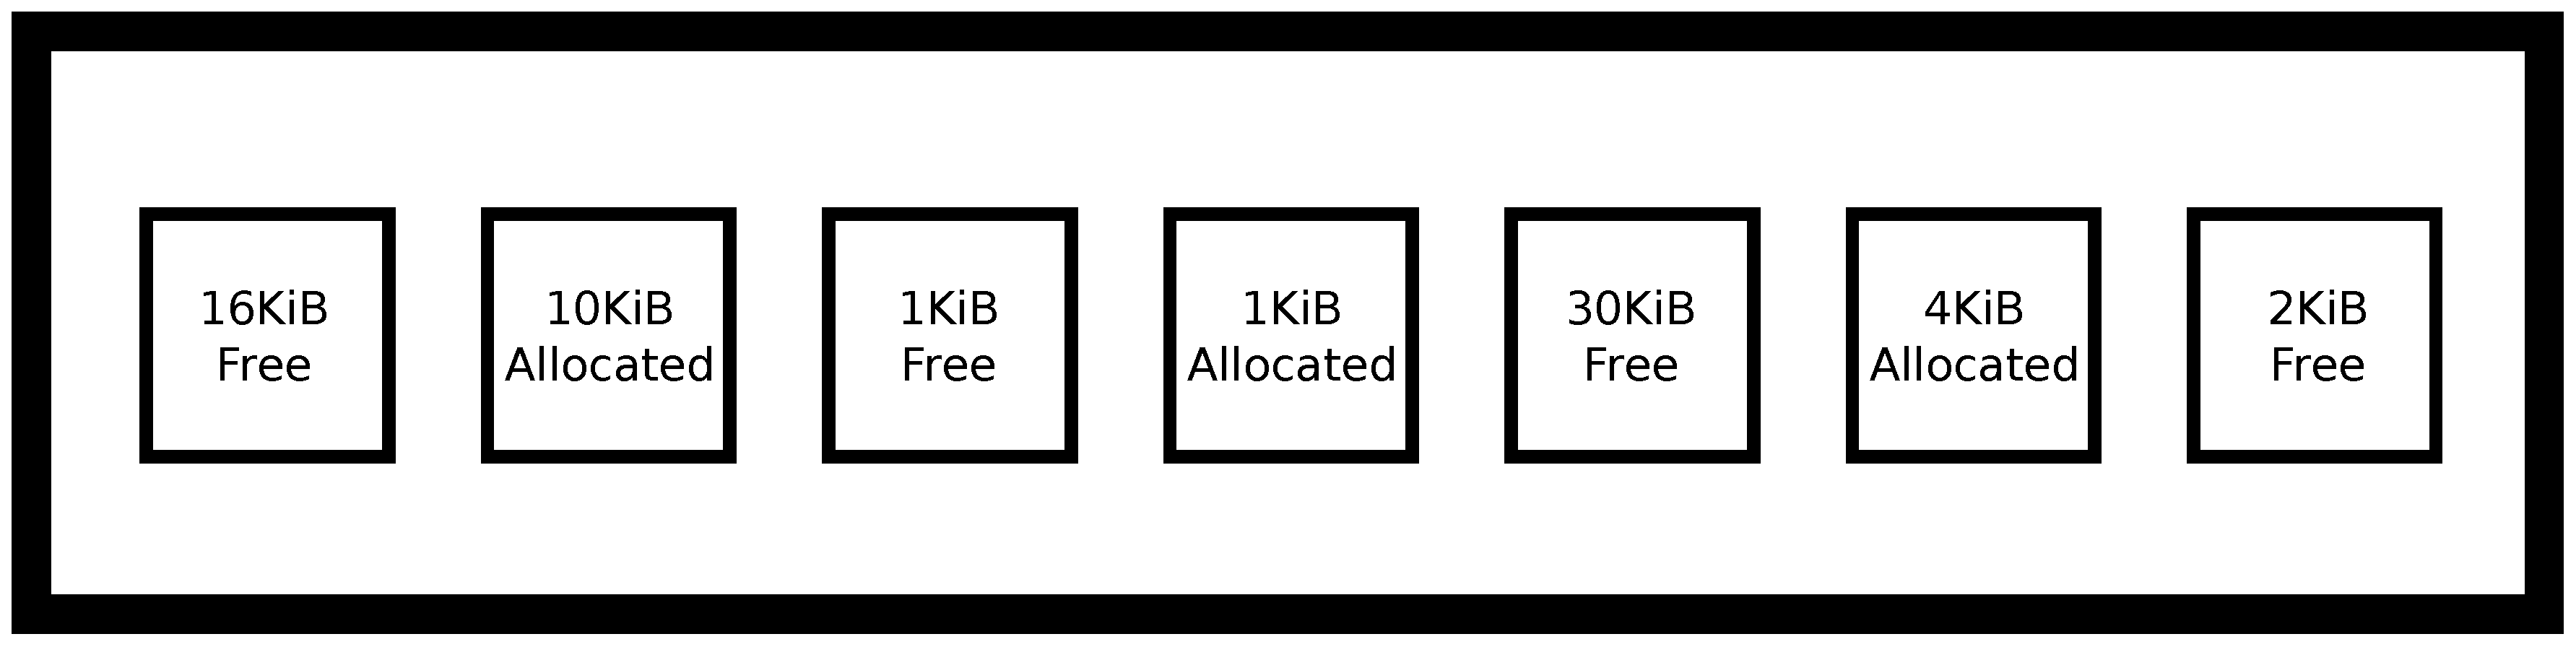
\includegraphics[width=.9\textwidth]{malloc/drawings/heap_empty.eps}
\caption{Empty heap blocks}
\end{figure}

If a new malloc request for 2KiB is executed (\keyword{malloc(2048)}), where should \keyword{malloc} reserve the memory?
It could use the last 2KiB hole, which happens to be the perfect size!
Or it could split one of the other two free holes.
These choices represent different placement strategies.
Whichever hole is chosen, the allocator will need to split the hole into two.
The newly allocated space, which will be returned to the program and a smaller hole if there is spare space left over.
A perfect-fit strategy finds the smallest hole that is of sufficient size (at least 2KiB):

\begin{figure}[H]
\centering
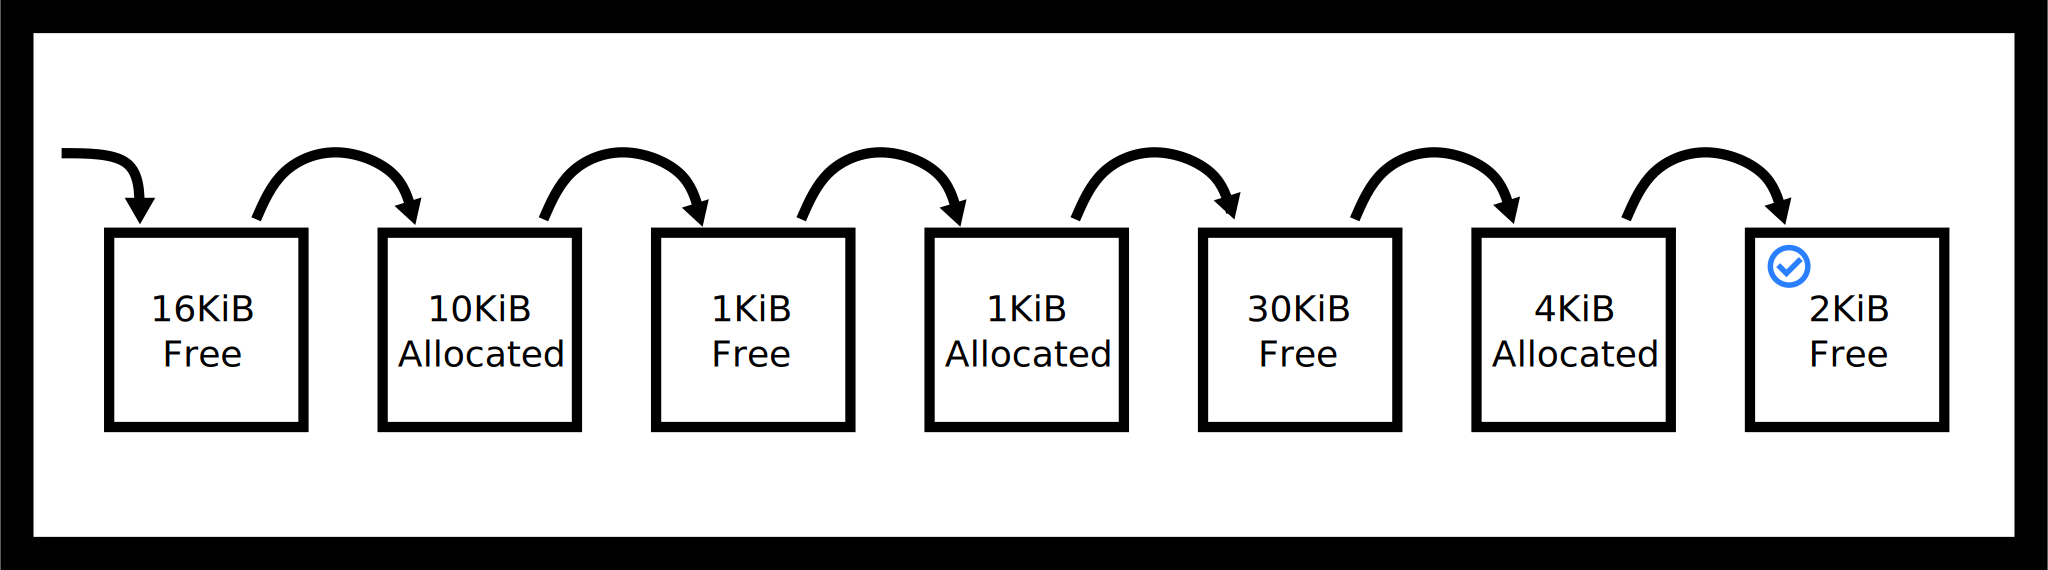
\includegraphics[width=.9\textwidth]{malloc/drawings/heap_best_fit.eps}
\caption{Best fit finds an exact match}
\end{figure}

A worst-fit strategy finds the largest hole that is of sufficient size so break the 30KiB hole into two:

\begin{figure}[H]
\centering
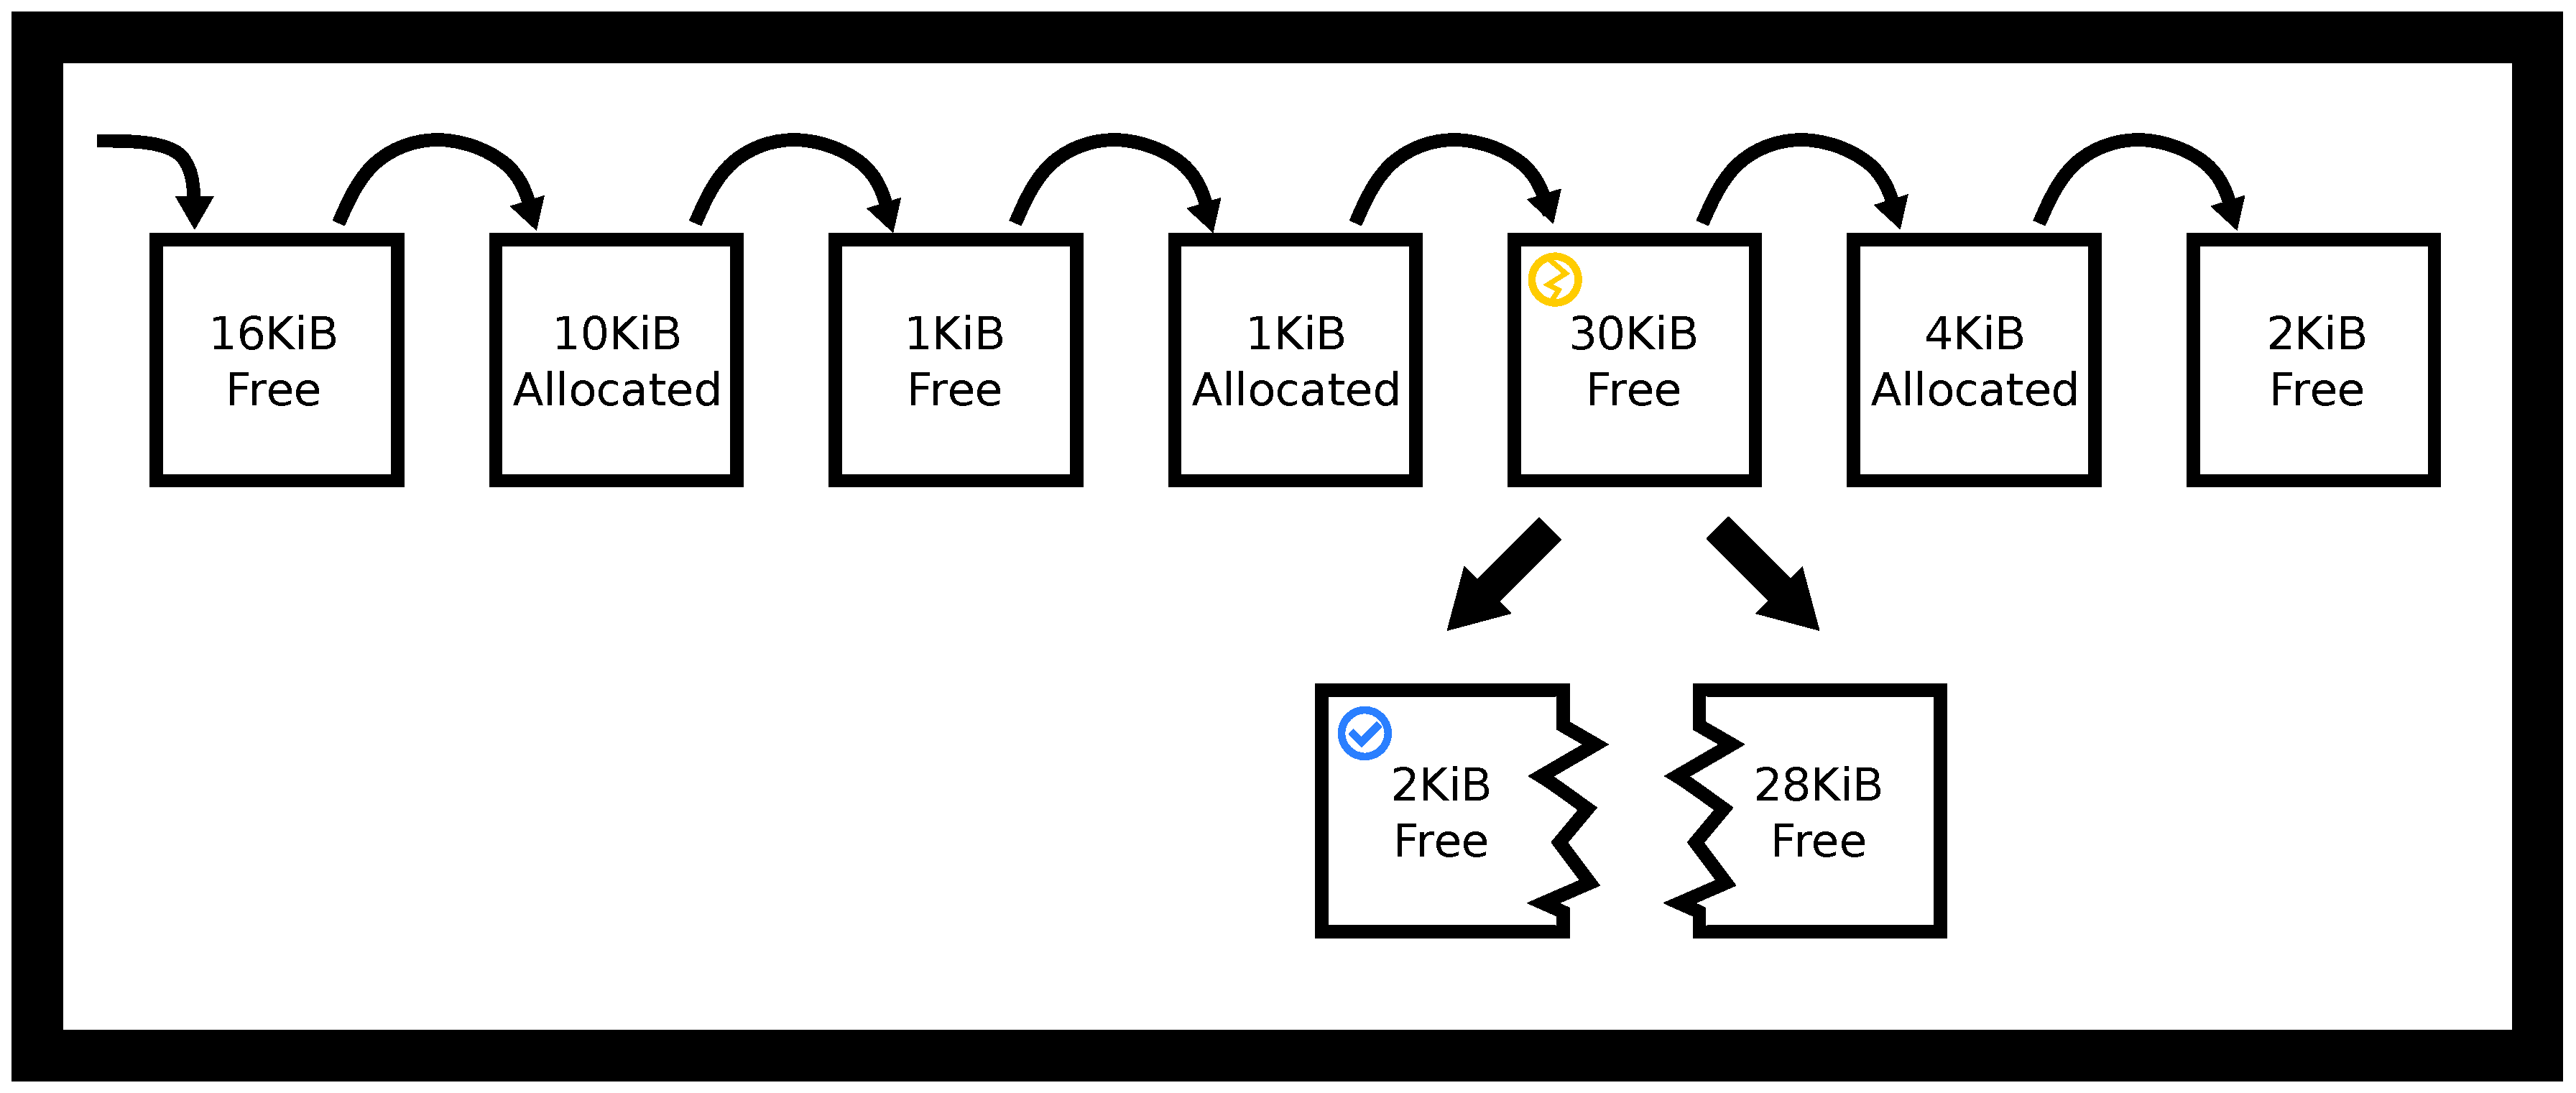
\includegraphics[width=.9\textwidth]{malloc/drawings/heap_worst_fit.eps}
\caption{Worst fit finds the worst match}
\end{figure}


A first-fit strategy finds the first available hole that is of sufficient size so break the 16KiB hole into two.
We don't even have to look through the entire heap!

\begin{figure}[H]
\centering
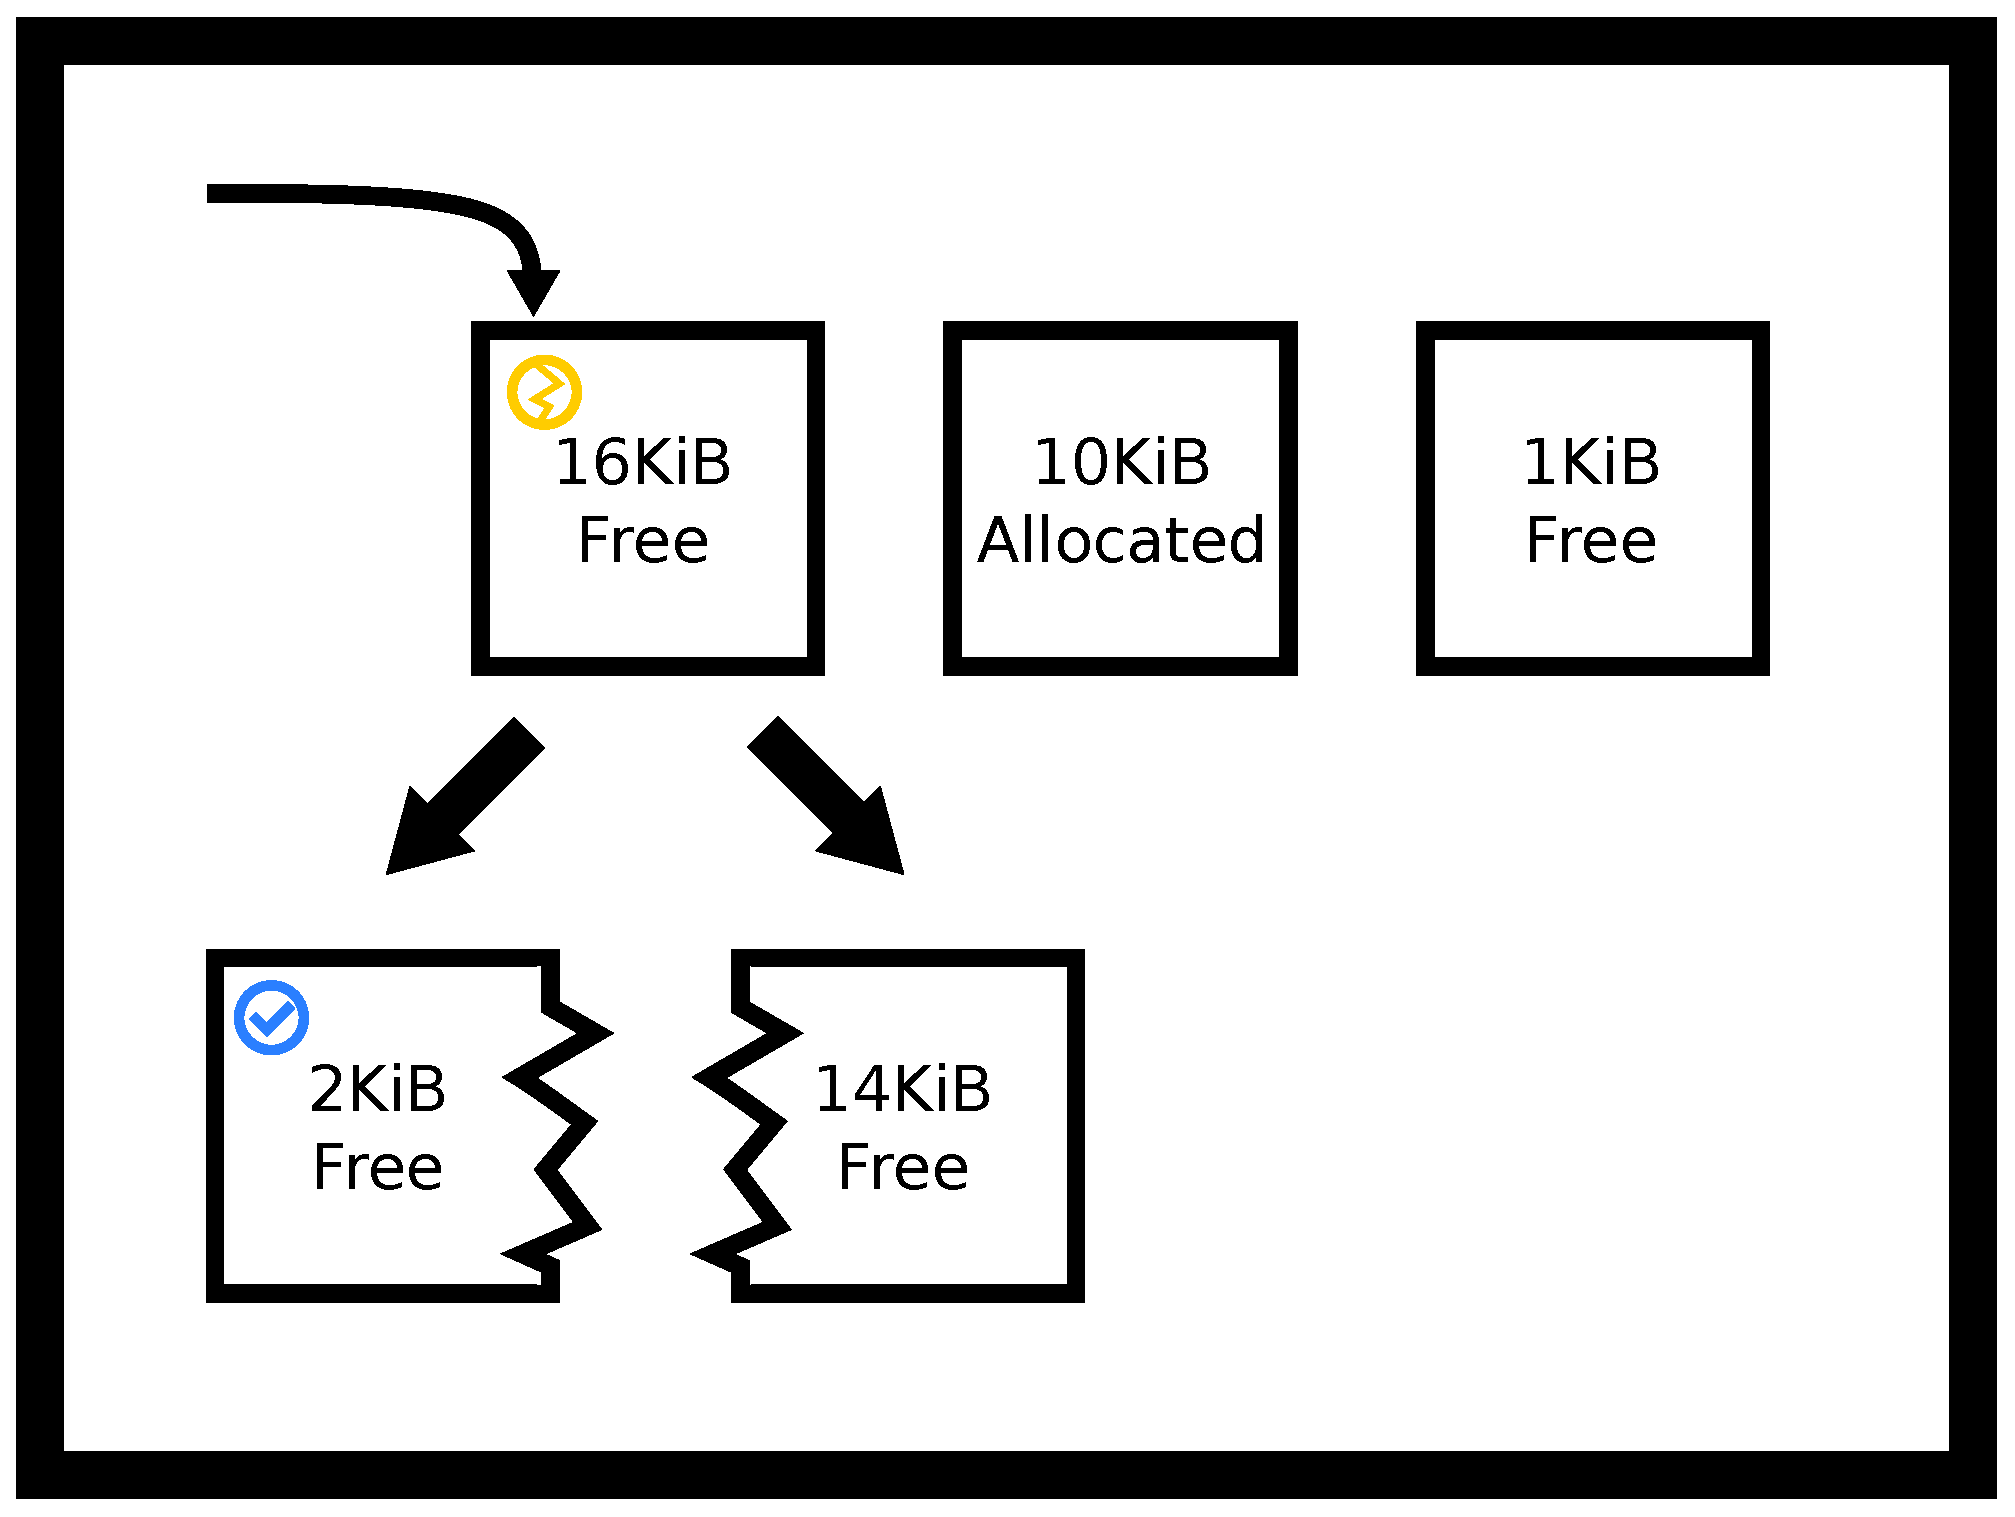
\includegraphics[width=.5\textwidth]{malloc/drawings/heap_first_fit.eps}
\caption{First fit finds the first match}
\end{figure}

One thing to keep in mind is that placement strategies don't need to replace the block.
For example, our first fit allocator could've just returned the original block unbroken.
Notice that this would lead to about 14KiB of space to be unused by the user and the allocator.
We call this internal fragmentation.

To introduce another concept, external fragmentation is that even though we have enough memory in the heap, it may be divided up in a way that we are not able to give the full amount.
In our previous example, of the 64KiB of heap memory, 17KiB is allocated, and 47KiB is free.
However, the largest available block is only 30KiB because our available unallocated heap memory is fragmented into smaller pieces.

\subsection{Placement Strategy Pros and Cons}

The challenges of writing a heap allocator are
\begin{itemize}
\item Need to minimize fragmentation (i.e.~maximize memory utilization)
\item Need high performance
\item Fiddly implementation -- lots of pointer manipulation using linked lists and pointer arithmetic.
\item Both fragmentation and performance depends on the application allocation profile, which can be evaluated but not predicted and in practice, under-specific usage conditions, a special-purpose allocator can often out-perform a general purpose implementation.
\item The allocator doesn't know the program's memory allocation requests in advance. Even if we did, this is the \href{http://en.wikipedia.org/wiki/Knapsack_problem}{Knapsack problem} which is known to be NP hard!
\end{itemize}

Different strategies affect the fragmentation of heap memory in non-obvious ways, which only are discovered by mathematical analysis or careful simulations under real-world conditions (for example simulating the memory allocation requests of a database or web server).

First we will have a more mathematical, one-shot approach to each of these algorithms \cite{Garey:1972:WAM:800152.804907}. The paper describes a scenario where you have a certain number of bins, and a certain number of allocations, and you are trying to fit the allocations in as few bins as possible, hence using as little memory as possible.
The paper discusses theoretical implications and puts a nice limit on the ratios in the long run between the ideal memory usage and the actual memory usage.
For those who are interested, the paper concludes that actual memory usage over ideal memory usage as the number of bins increases -- the bins can have any distribution -- is about 1.7 for first fit and lower bounded by 1.7 for best fit.
The problem with this analysis is that very few real world applications need this type of one-shot allocation.
Video game object allocations will typically designate a different subheap for each level and fill up that subheap if they need a quick memory allocation scheme that they can throw away.

In practice, we'll be using the result from a more rigorous survey conducted in 2005 \cite{10.1007/3-540-60368-9_19}.
The survey makes sure to note that memory allocation is a moving target.
A good allocation scheme to one program may not be a good allocation scheme to another program.
Programs don't uniformly follow the distribution of allocations, so very.
The survey talks about all the allocation schemes that we have introduced as well as a few extra ones.
Here are some summarized takeaways

\begin{enumerate}
\item Best fit may have problems when a block is chosen that is almost the right size, and the remaining space is split so small that a program probably won't use it.
  A way to get around this could be to set a threshold for splitting.
  This small splitting isn't observed as frequently under regular workload.
  In addition, the worst case behavior of best fit is bad, but doesn't usually happen p. 43.
\item The survey also talks about an important distinction of first fit.
  There are multiple notions of first.
  First could be ordered in terms of time of free, or it could be ordered through the addresses of the start of the block, or it could be ordered by the time of last free -- first being least recently used.
  The survey didn't go too in depth into the performance of each, but did make a note that address ordered and least recently used lists ended up with better performance than the most recently used first.
\item The survey concludes by first saying that under simulated random (assuming uniform at random) work loads, best fit and first fit do as well. Even in practice, both best and address ordered first fit do about as equally as well with a splitting threshold and coalescing. The reasons why aren't entirely known.
\end{enumerate}

Some additional notes we make

\begin{enumerate}
\item Best fit may not require a full scan of the heap. When a block of perfect size or of perfect size within a threshold is found, that can be returned, depending on what edge-case policy you have.
\item Worst fit may not need to scan the entire heap as well. Your heap could be represented with the max-heap data structure and each allocation call could simply pop the top off, reheapify, and possibly insert a split memory block.
  Using Fibonacci heaps, however, could be extremely inefficient.
\item First fit needs to have some sort of ordering. Most of the time people will default to linked lists which is a fine choice. There aren't too many improvements you can make with a least recently used and most recently used linked list policy, but with address ordered linked lists you can speed up insertion from O(n) to O(log(n)) by using a randomized skip-list in conjunction with your singly linked list.
  Basically an insert would use the skip list as shortcuts to find the right place to insert the block and a removal would go through the list as normal.
\item There are many placement strategies that we haven't talked about, one is next-fit which is first fit on the next fit block. This adds a sort-of deterministic randomness. You won't be expected to know this algorithm, just know as you are implementing a memory allocator as part of a machine problem, there are more than these.
  \end{enumerate}

\section{Memory Allocator Tutorial}

A memory allocator needs to keep track of which bytes are currently allocated and which are available for use.
This section introduces the implementation and conceptual details of building an allocator, or the actual code that implements \keyword{malloc} and \keyword{free}.

Conceptually, we are thinking about creating linked lists and lists of blocks!
Please enjoy the following ASCII art.
bt is short for boundary tag.


\begin{figure}[H]
\centering
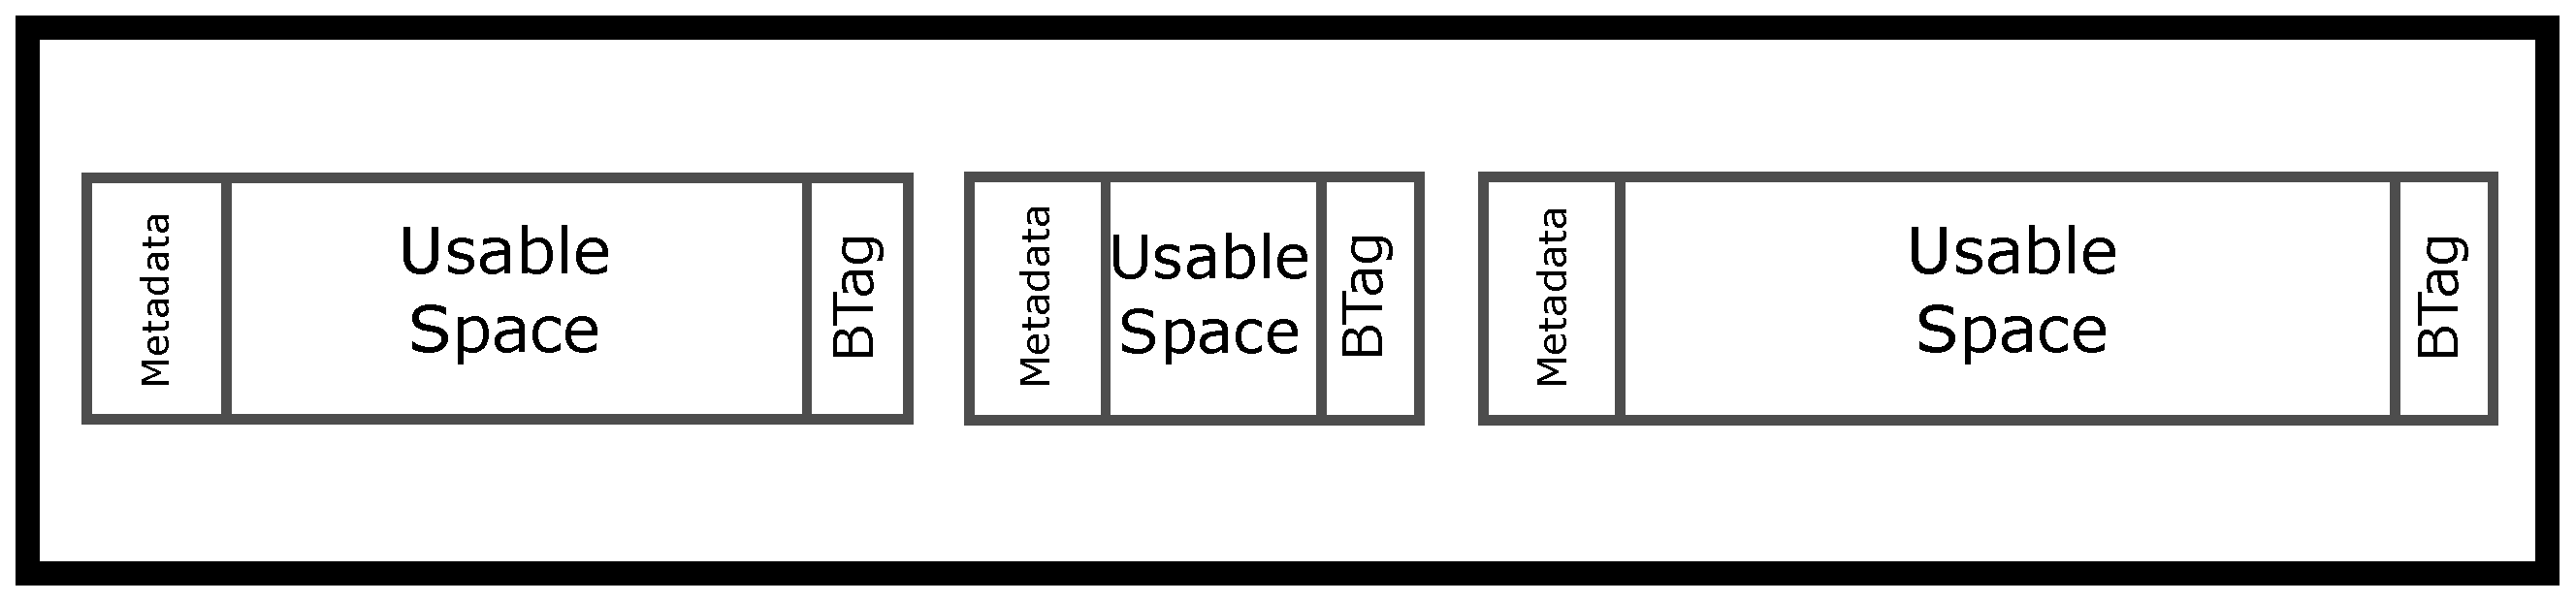
\includegraphics[width=.7\textwidth]{malloc/drawings/malloc_patching.eps}
\caption{3 Adjacent Memory blocks}
\end{figure}

We will have implicit pointers in our next block, meaning that we can get from one block to another using addition.
This is in contrast to an explicit \keyword{metadata *next} field in our meta block.

\begin{figure}[H]
\centering
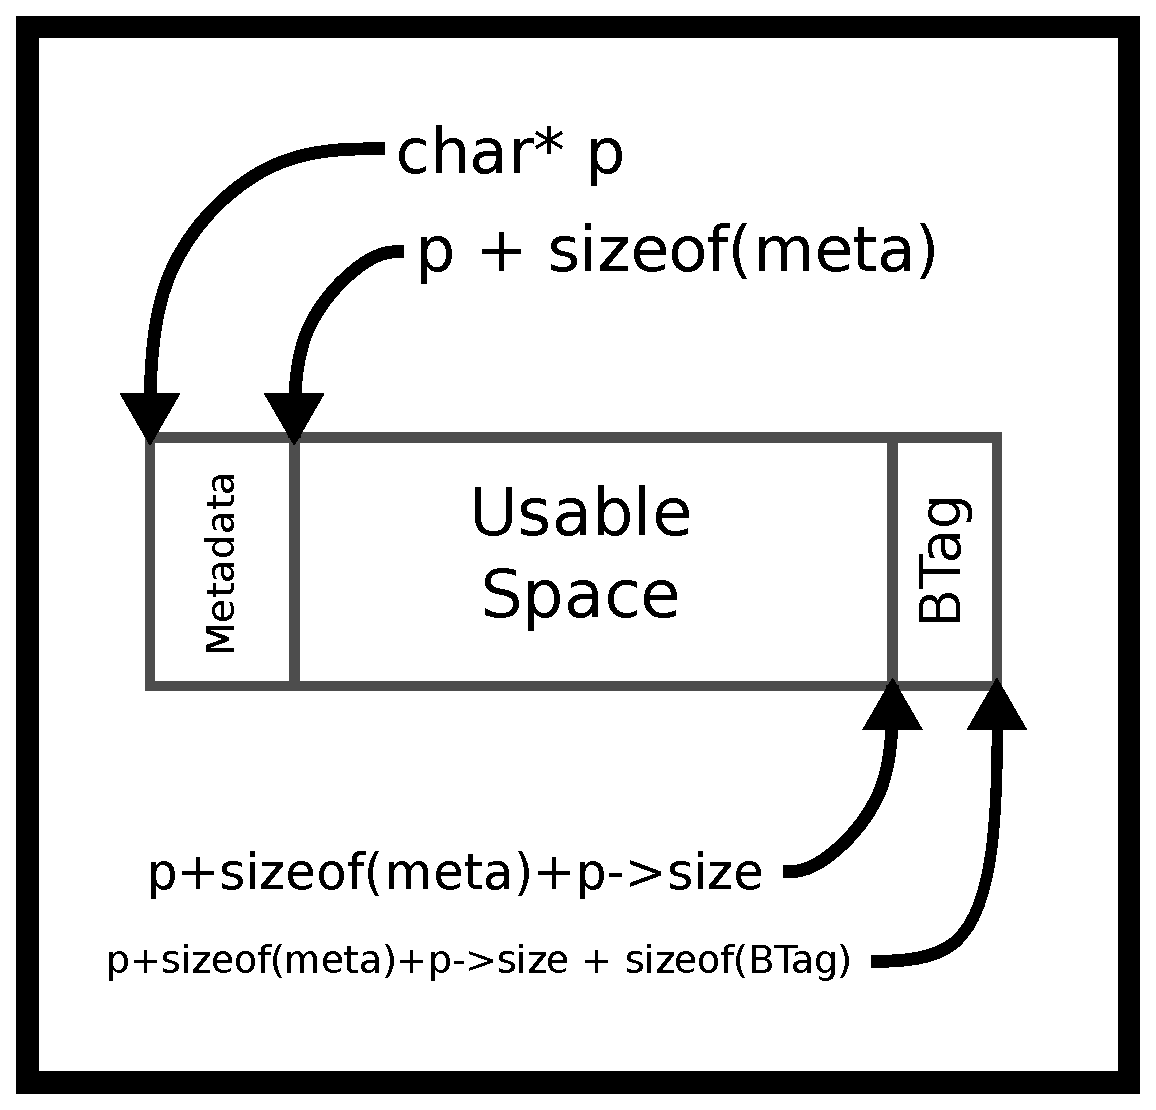
\includegraphics[width=.5\textwidth]{malloc/drawings/malloc_addition.eps}
\caption{Malloc addition}
\end{figure}

One can grab the next block by finding the end of the current one.
That is what we mean by ``implicit list''.

The actual spacing may be different.
The metadata can contain different things.
A minimal metadata would simply have the size of the block.

Since we write integers and pointers into memory that we already control, we can later consistently hop from one address to the next.
This internal information represents some overhead.
Meaning even if we had requested 1024 KiB of contiguous memory from the system, we will not be able to provide all of it to the running program.

Our heap memory is a list of blocks where each block is either allocated or unallocated.
Thus there is conceptually a list of free blocks, but it is implicit in the form of block size information that we store as part of each block.
Let's think of it in terms of a simple implementation.
\begin{lstlisting}[language=C]
typedef struct {
  size_t block_size;
  char data[0];
} block;
block *p = sbrk(100);
p->size = 100 - sizeof(*p) - sizeof(BTag);
// Other block allocations
\end{lstlisting}

We could navigate from one block to the next block just by adding the block's size.

\begin{lstlisting}[language=C]
p + sizeof(metadata) + p->block_size + sizeof(BTag)
\end{lstlisting}

Make sure to get your casting right!
Otherwise you will move an extreme amount of bytes over.

The calling program never sees these values.
They are internal to the implementation of the memory allocator.
As an example, suppose your allocator is asked to reserve 80 bytes (\keyword{malloc(80)}) and requires 8 bytes of internal header data.
The allocator would need to find an unallocated space of at least 88 bytes.
After updating the heap data it would return a pointer to the block.
However, the returned pointer does not point to the start of the block because that's where the internal size data is stored!
Instead we would return the start of the block + 8 bytes.
In the implementation, remember that pointer arithmetic depends on type. For example, \keyword{p\ +=\ 8} adds \keyword{8\ *\ sizeof(p)}, not necessarily 8 bytes!

\subsection{Implementing malloc}

The simplest implementation uses first fit.
Start at the first block, assuming it exists, and iterate until a block that represents unallocated space of sufficient size is found, or we've checked all the blocks.
If no suitable block is found, it's time to call \keyword{sbrk()} again to sufficiently extend the size of the heap.
For the purposes of this class, we will try to serve every memory request until the operating system tells us we are going to run out of heap space.
Other applications may limit themselves to a certain heap size and cause requests to intermittently fail.
In addition, a fast implementation might extend it a significant amount so that we will not need to request more heap memory in the near future.

When a free block is found, it may be larger than the space we need.
If so, we will create two entries in our implicit list.
The first entry is the allocated block, the second entry is the remaining space.
There are ways to do this if you want to keep the overhead small.
We recommend first for going with readability.

\begin{lstlisting}[language=C]
typedef struct {
  size_t block_size;
  int is_free;
  char data[0];
} block;
block *p = sbrk(100);
p->size = 100 - sizeof(*p) - sizeof(boundary_tag);
// Other block allocations
\end{lstlisting}

If you want certain bits to hold different pieces of information, use bit fields!

\begin{lstlisting}[language=C]
typedef struct {
  unsigned int block_size : 7;
  unsigned int is_free : 1;
} size_free;

typedef struct {
  size_free info;
  char data[0];
} block;
\end{lstlisting}

The compiler will handle it for you.
After setting up your fields then it becomes simply looping through each of the blocks and checking the appropriate fields

Here is a visual representation of what happens.
As for some more ascii art, if we assume that we have a block that looks like this, we want to spit if the allocation is let's say 16 bytes
The split we'll have to do is the following.

\begin{figure}[H]
\centering
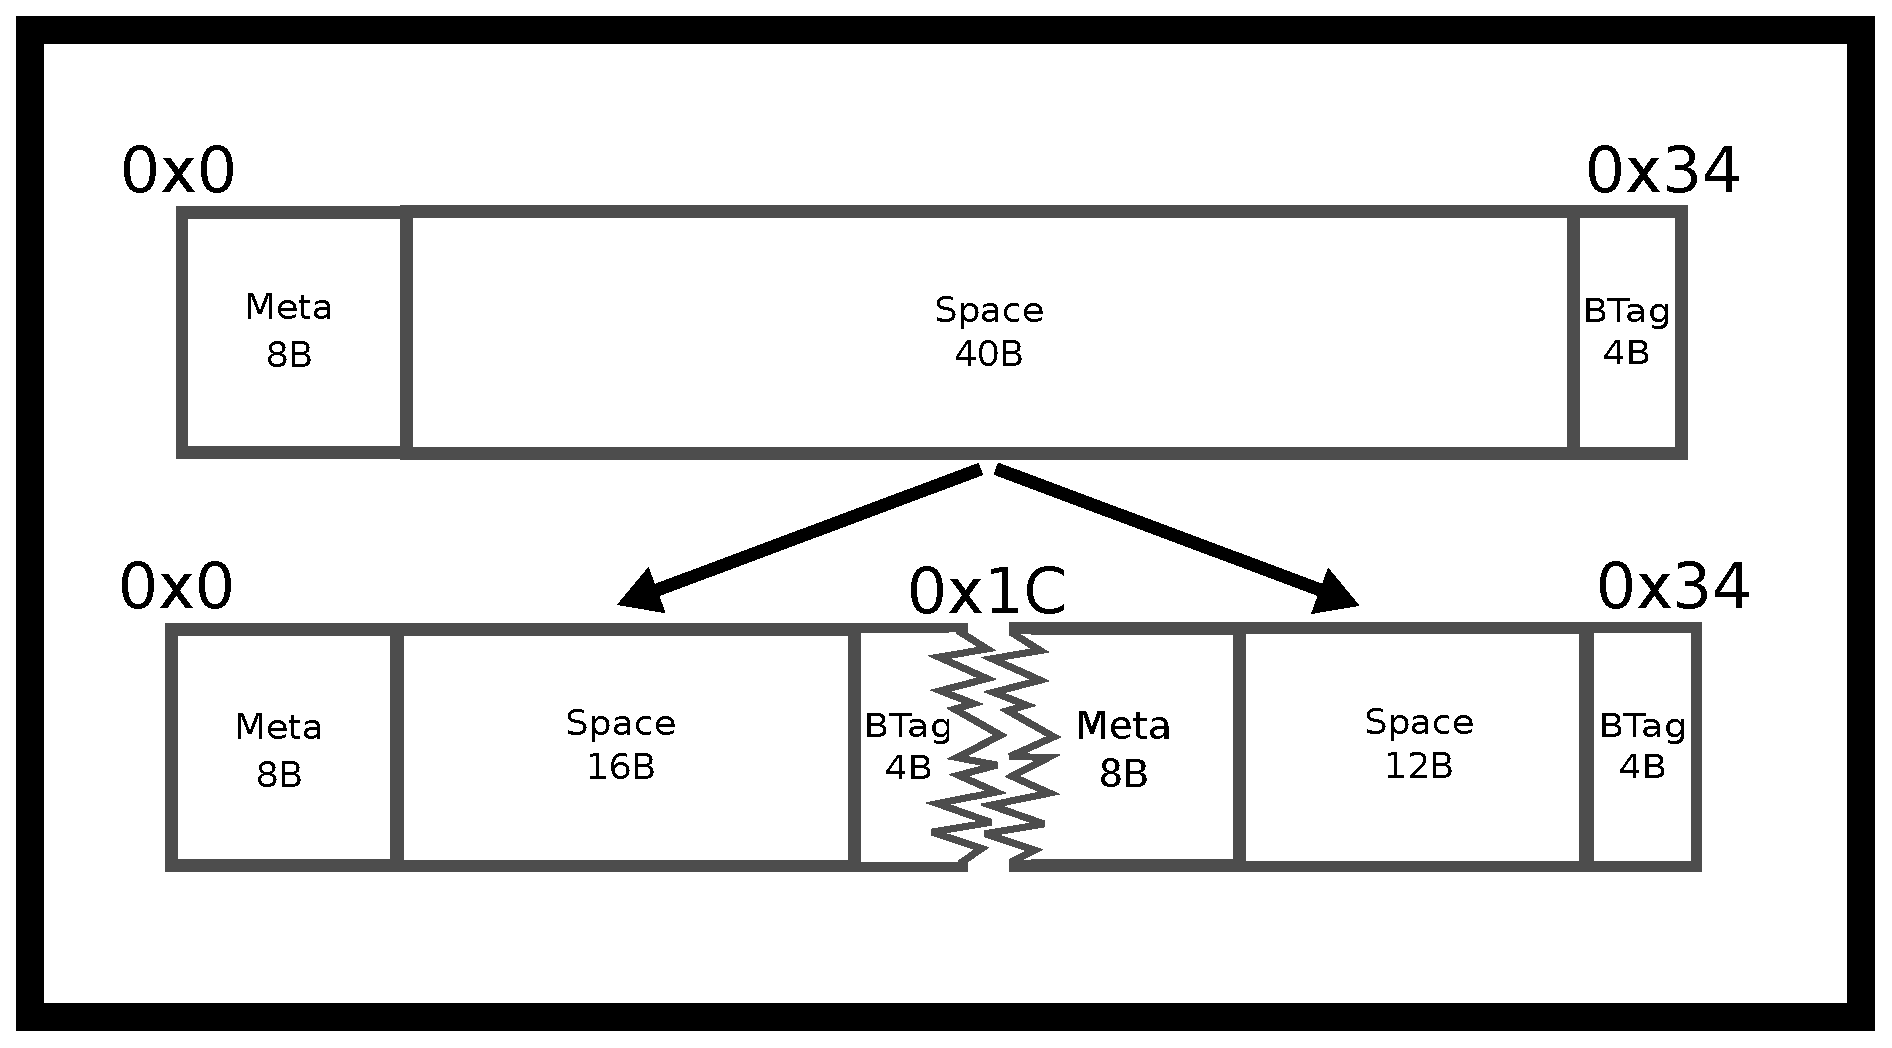
\includegraphics[width=.7\textwidth]{malloc/drawings/malloc_split.eps}
\caption{Malloc split}
\end{figure}

This is before alignment concerns as well.

\subsection{Alignment and rounding up considerations}

Many architectures expect multibyte primitives to be aligned to some multiple of 2 (4, 16, etc).
For example, it's common to require 4-byte types to be aligned to 4-byte boundaries and 8-byte types on 8-byte boundaries.
If multi-byte primitives are not stored on a reasonable boundary for example starting at an odd address then the performance can be significantly impacted because it may require two memory read requests instead of one.
On some architectures the penalty is even greater - the program will crash with a \href{http://en.wikipedia.org/wiki/Bus_error\#Unaligned_access}{bus error}.
Most of you have experienced this in your architecture classes if there was no memory protection.

As \keyword{malloc} does not know how the user will use the allocated memory, the pointer returned to the program needs to be aligned for the worst case, which is architecture dependent.

From glibc documentation, the glibc \keyword{malloc} uses the following heuristic \cite{vma_paging}

\begin{quote}
The block that malloc gives you is guaranteed to be aligned so that it can hold any type of data. On GNU systems, the address is always a multiple of eight on most systems, and a multiple of 16 on 64-bit systems." For example, if you need to calculate how many 16 byte units are required, don't forget to round up.
\end{quote}

This is what the math would look like in C.

\begin{lstlisting}[language=C]
int s = (requested_bytes + tag_overhead_bytes + 15) / 16
\end{lstlisting}

The additional constant ensures incomplete units are rounded up. Note, real code is more likely to symbol sizes e.g. \keyword{sizeof(x)\ -\ 1}, rather than coding numerical constant 15.
\href{http://www.ibm.com/developerworks/library/pa-dalign/}{Here's a great article on memory alignment, if you are further interested}

Another added effect is could be internal fragmentation happens when the block you give them is larger than their allocation size.
Let's say that we have a free block of size 16B (not including metadata).
If they allocate 7 bytes, you may want to round up to 16B and just return the entire block.
This gets very sinister when you implementing coalescing and splitting.
If you don't implement either, then you may end up returning a block of size 64B for a 7B allocation!
There is a \emph{lot} of overhead for that allocation which is what we are trying to avoid.

\subsection{Implementing free}

When \keyword{free} is called we need to re-apply the offset to get back to the `real' start of the block -- to where we stored the size information.
A naive implementation would simply mark the block as unused.
If we are storing the block allocation status in a bit field, then we just need to clear the bit:

\begin{lstlisting}[language=C]
p->info.is_free = 0;
\end{lstlisting}

However, we have a bit more work to do.
If the current block and the next block (if it exists) are both free we need to coalesce these blocks into a single block.
Similarly, we also need to check the previous block, too.
If that exists and represents an unallocated memory, then we need to coalesce the blocks into a single large block.

To be able to coalesce a free block with a previous free block we will also need to find the previous block, so we store the block's size at the end of the block, too.
These are called ``boundary tags'' \cite{knuth1973art}.
These are Knuth's solution to the coalescing problem both ways.
As the blocks are contiguous, the end of one block sits right next to the start of the next block.
So the current block (apart from the first one) can look a few bytes further back to lookup the size of the previous block.
With this information you can now jump backwards!

Take for example a double coalesce.
If we wanted to free the middle block we need to turn the surrounding blocks into one big blocks

\begin{figure}[H]
\centering
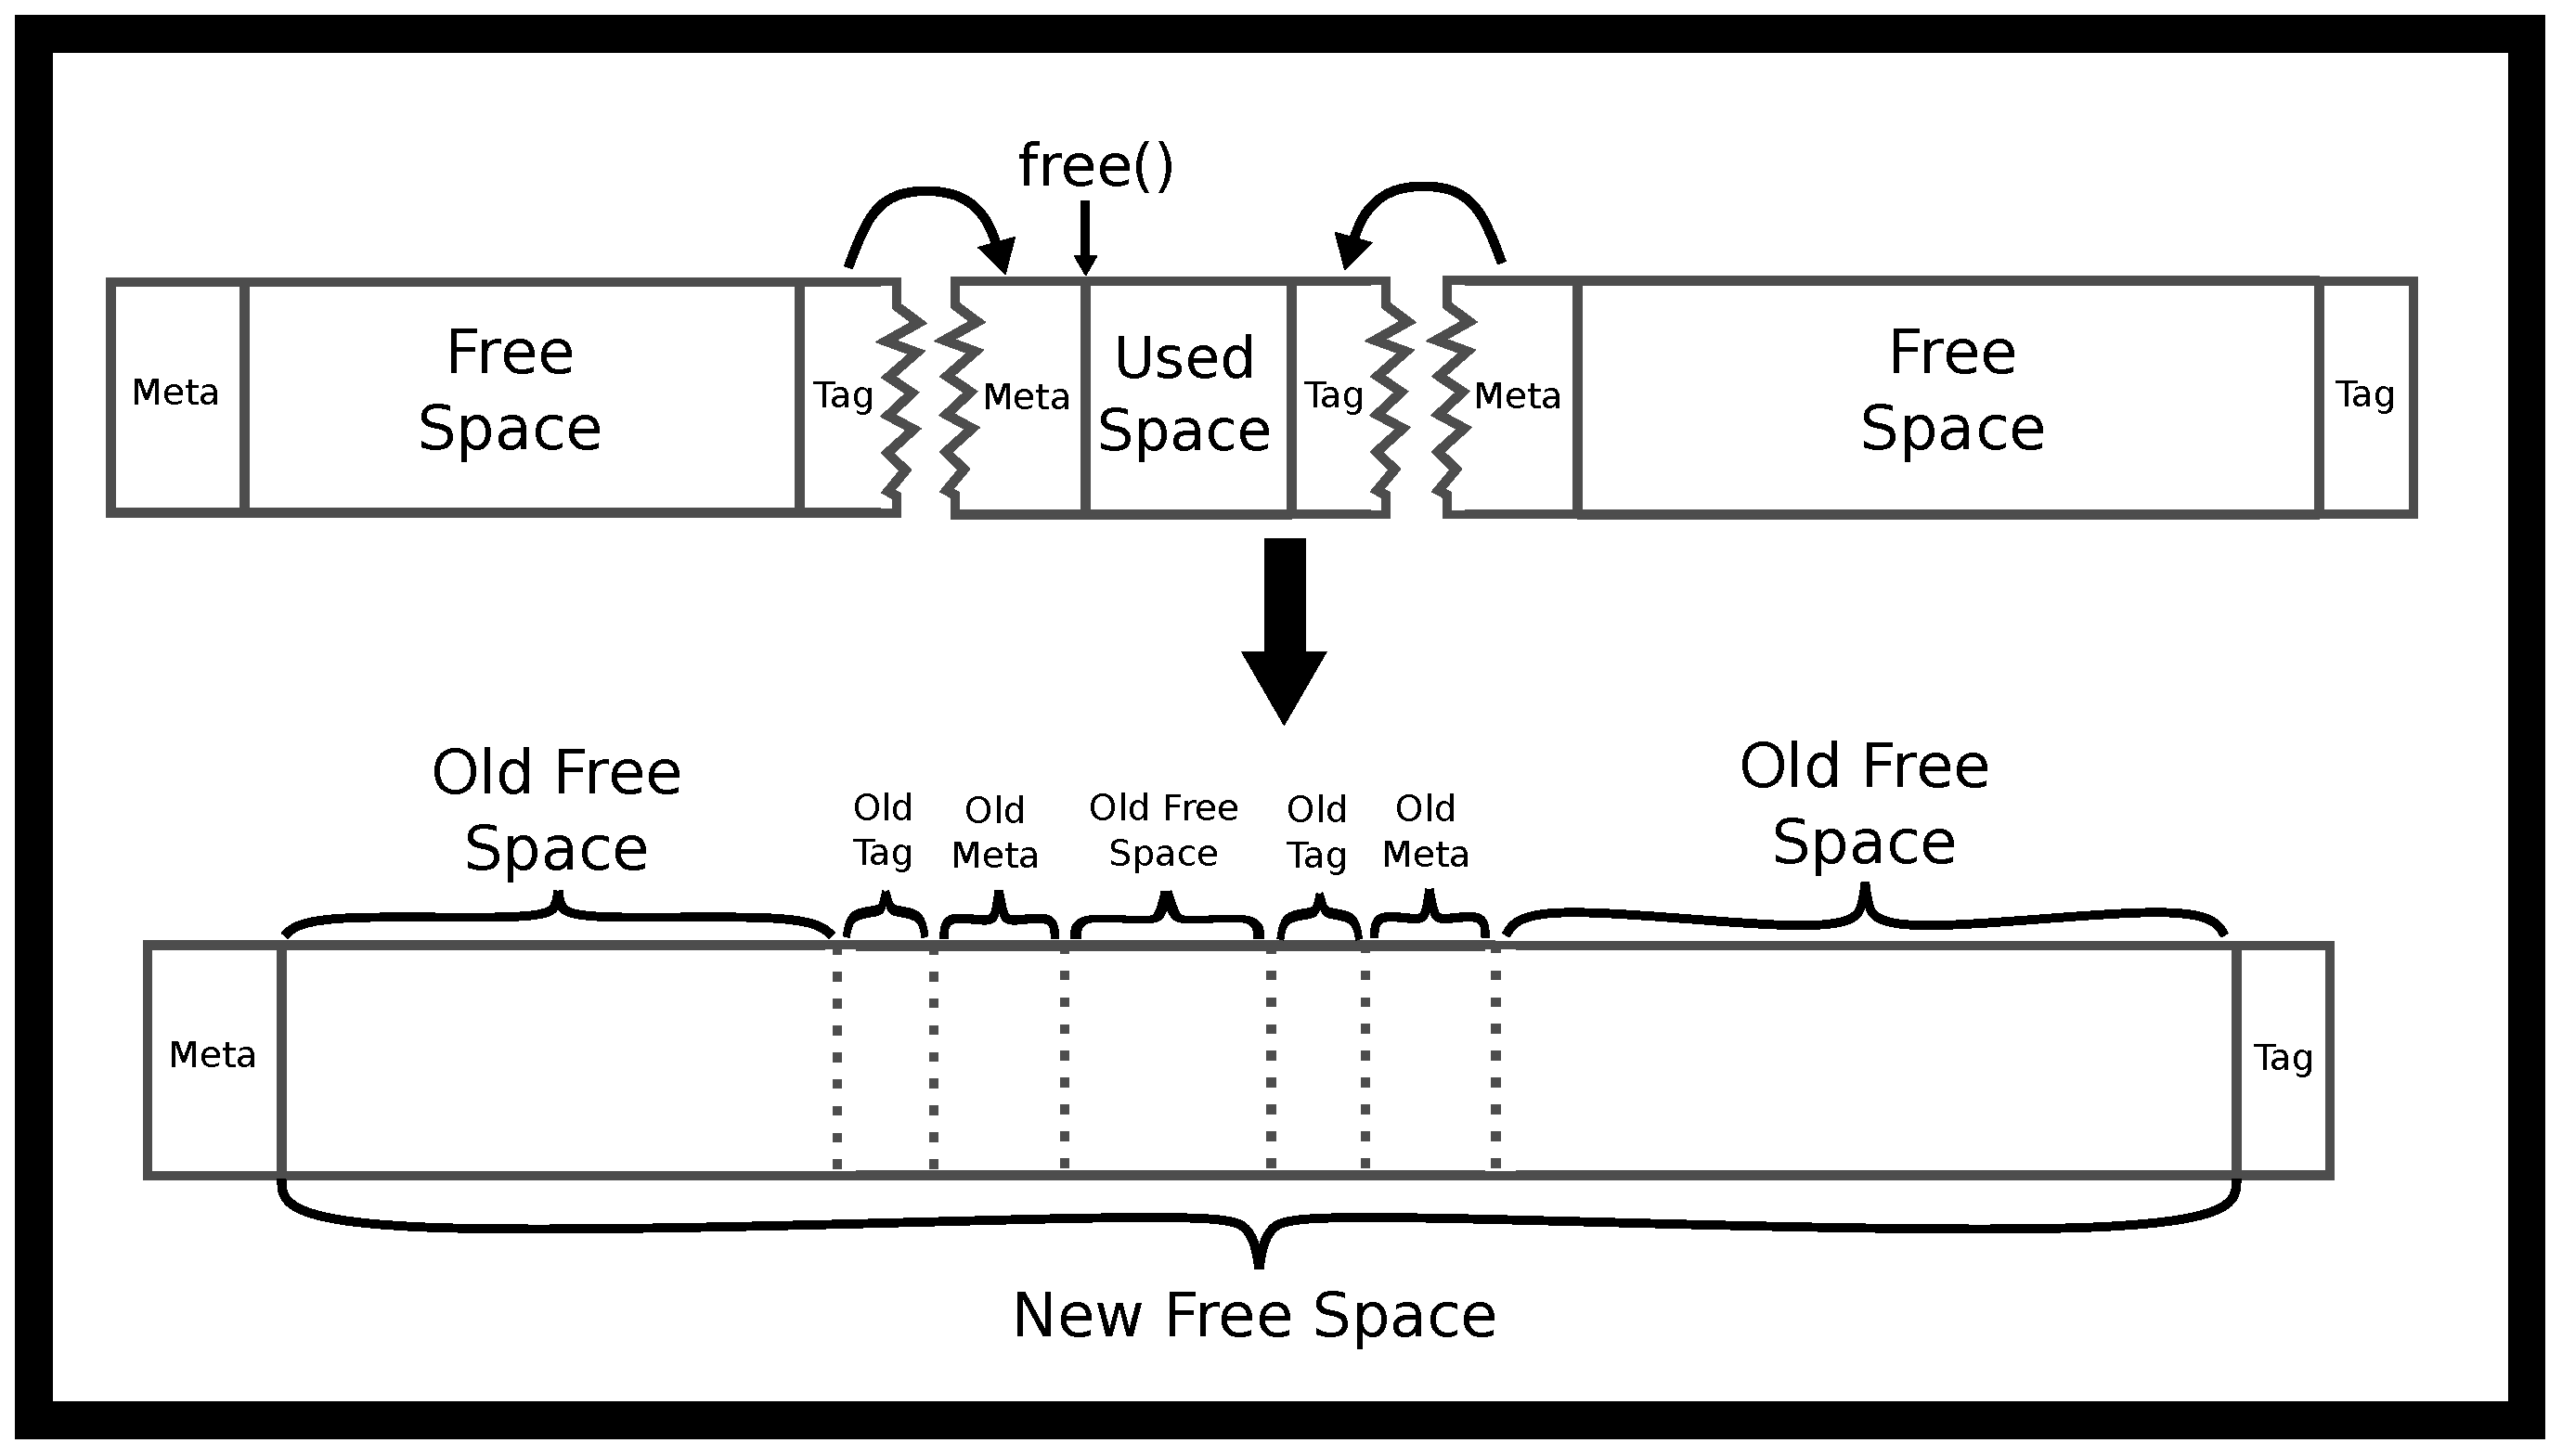
\includegraphics[width=.9\textwidth]{malloc/drawings/malloc_double_coalesce.eps}
\caption{Free double coalesce}
\end{figure}

\subsection{Performance}

With the above description it's possible to build a memory allocator.
It's main advantage is simplicity - at least simple compared to other allocators!
Allocating memory is a worst-case linear time operation -- search linked lists for a sufficiently large free block.
De-allocation is constant time.
No more than 3 blocks will need to be coalesced into a single block, and using a most recently used block scheme only one linked list entry.

Using this allocator it is possible to experiment with different placement strategies.
For example, you could start searching from where you last deallocated a block, or where you last allocated from.
If you do store pointers to blocks, you need to be very careful that they always remain valid
Particularly when you malloc, free, calloc, realloc, coalesce, split, etc.

\subsection{Explicit Free Lists Allocators}

Better performance can be achieved by implementing an explicit doubly-linked list of free nodes.
In that case, we can immediately traverse to the next free block and the previous free block.
This can reduce the search time, because the linked list only includes unallocated blocks.
A second advantage is that we now have some control over the ordering of the linked list.
For example, when a block is deallocated, we could choose to insert it into the beginning of the linked list rather than always between its neighbors.
We may update our struct to look like this

\begin{lstlisting}[language=C]
typedef struct {
  size_t info;
  struct block *next;
  char data[0];
} block;
\end{lstlisting}

Here is what that would look like along with our implicit linked list

\begin{figure}[H]
\centering
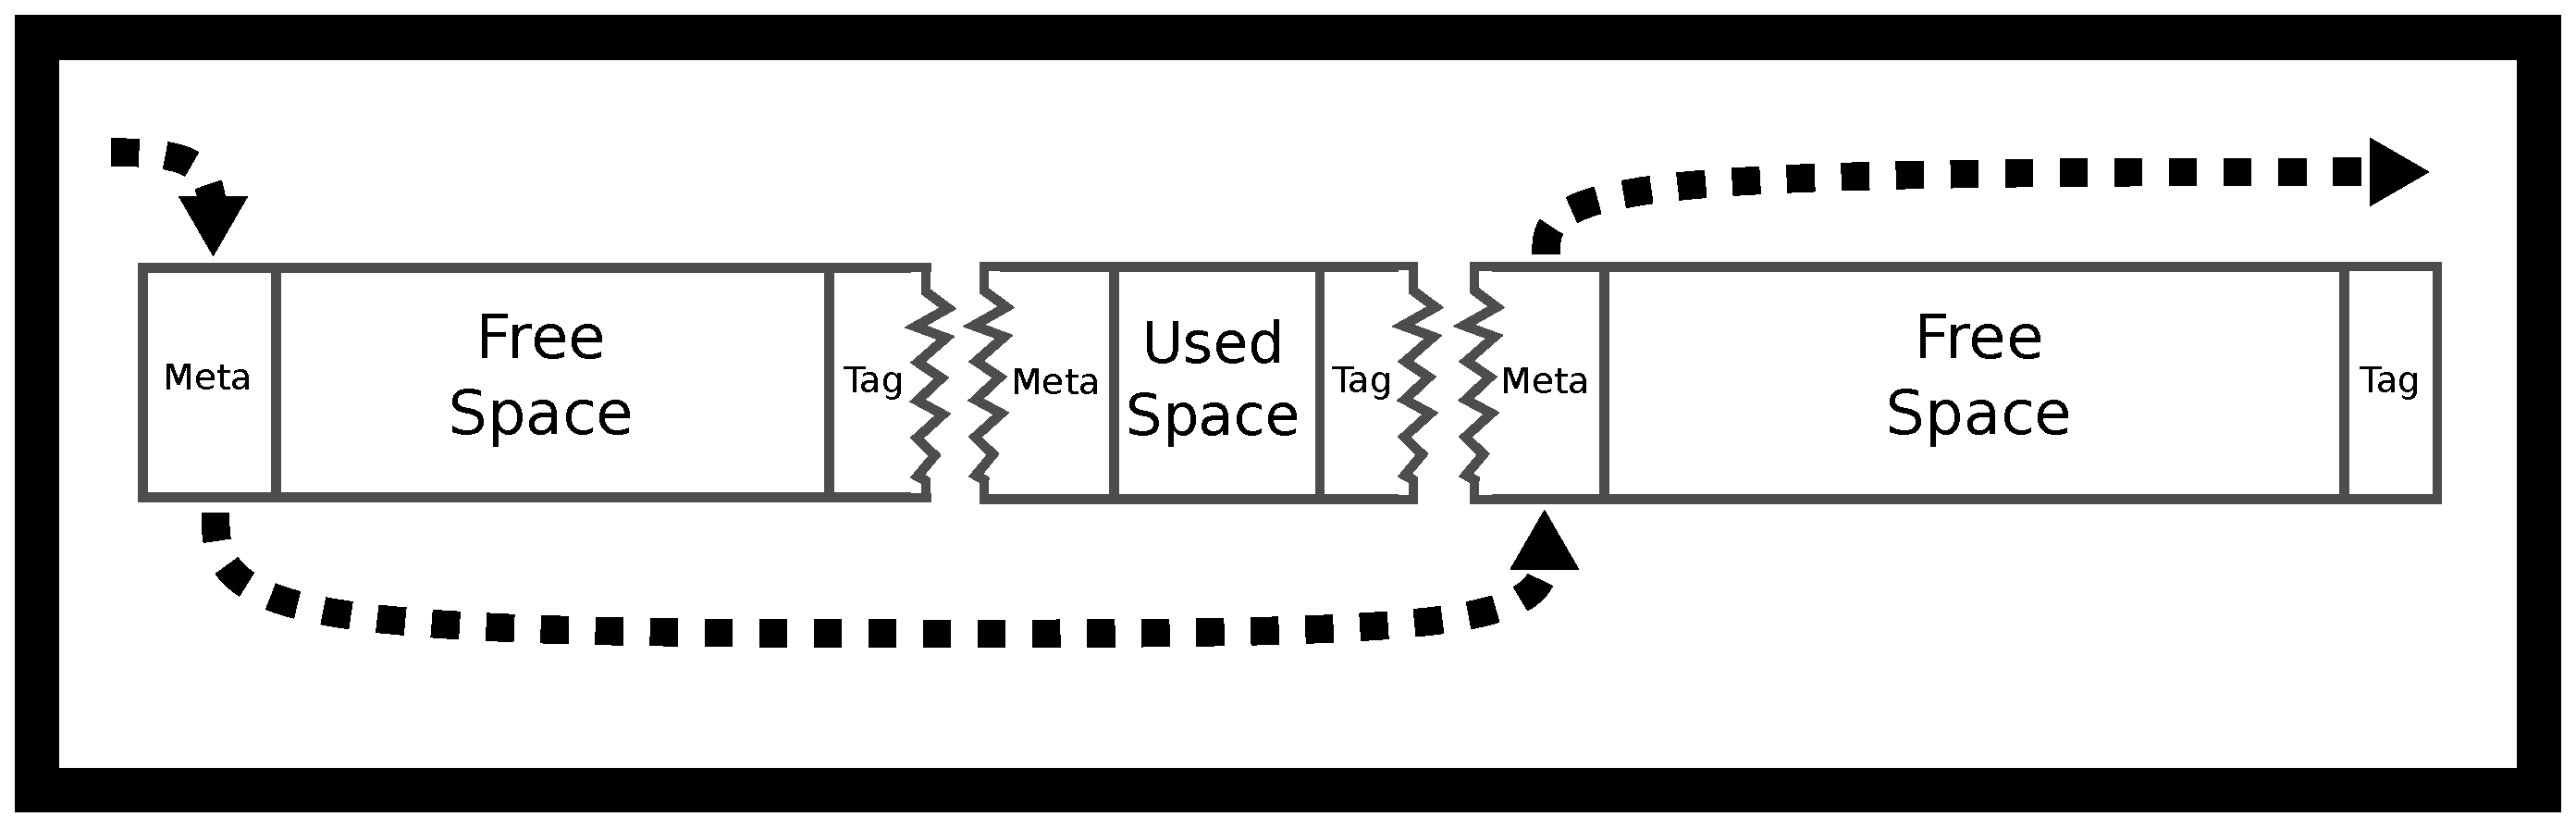
\includegraphics[width=.7\textwidth]{malloc/drawings/free_list.eps}
\caption{Free list}
\end{figure}


Where do we store the pointers of our linked list?
A simple trick is to realize that the block itself is not being used and store the next and previous pointers as part of the block, though now you have to ensure that the free blocks are always sufficiently large to hold two pointers.
We still need to implement Boundary Tags, so we can correctly free blocks and coalesce them with their two neighbors.
Consequently, explicit free lists require more code and complexity.
With explicit linked lists a fast and simple `Find-First' algorithm is used to find the first sufficiently large link.
However, since the link order can be modified, this corresponds to different placement strategies.
For example if the links are maintained from largest to smallest, then this produces a `Worst-Fit' placement strategy.

There are edge cases though, consider how you would maintain your free list if you also have to perform a double coalesce.
We've included a figure with a common mistake.

\begin{figure}[H]
\centering
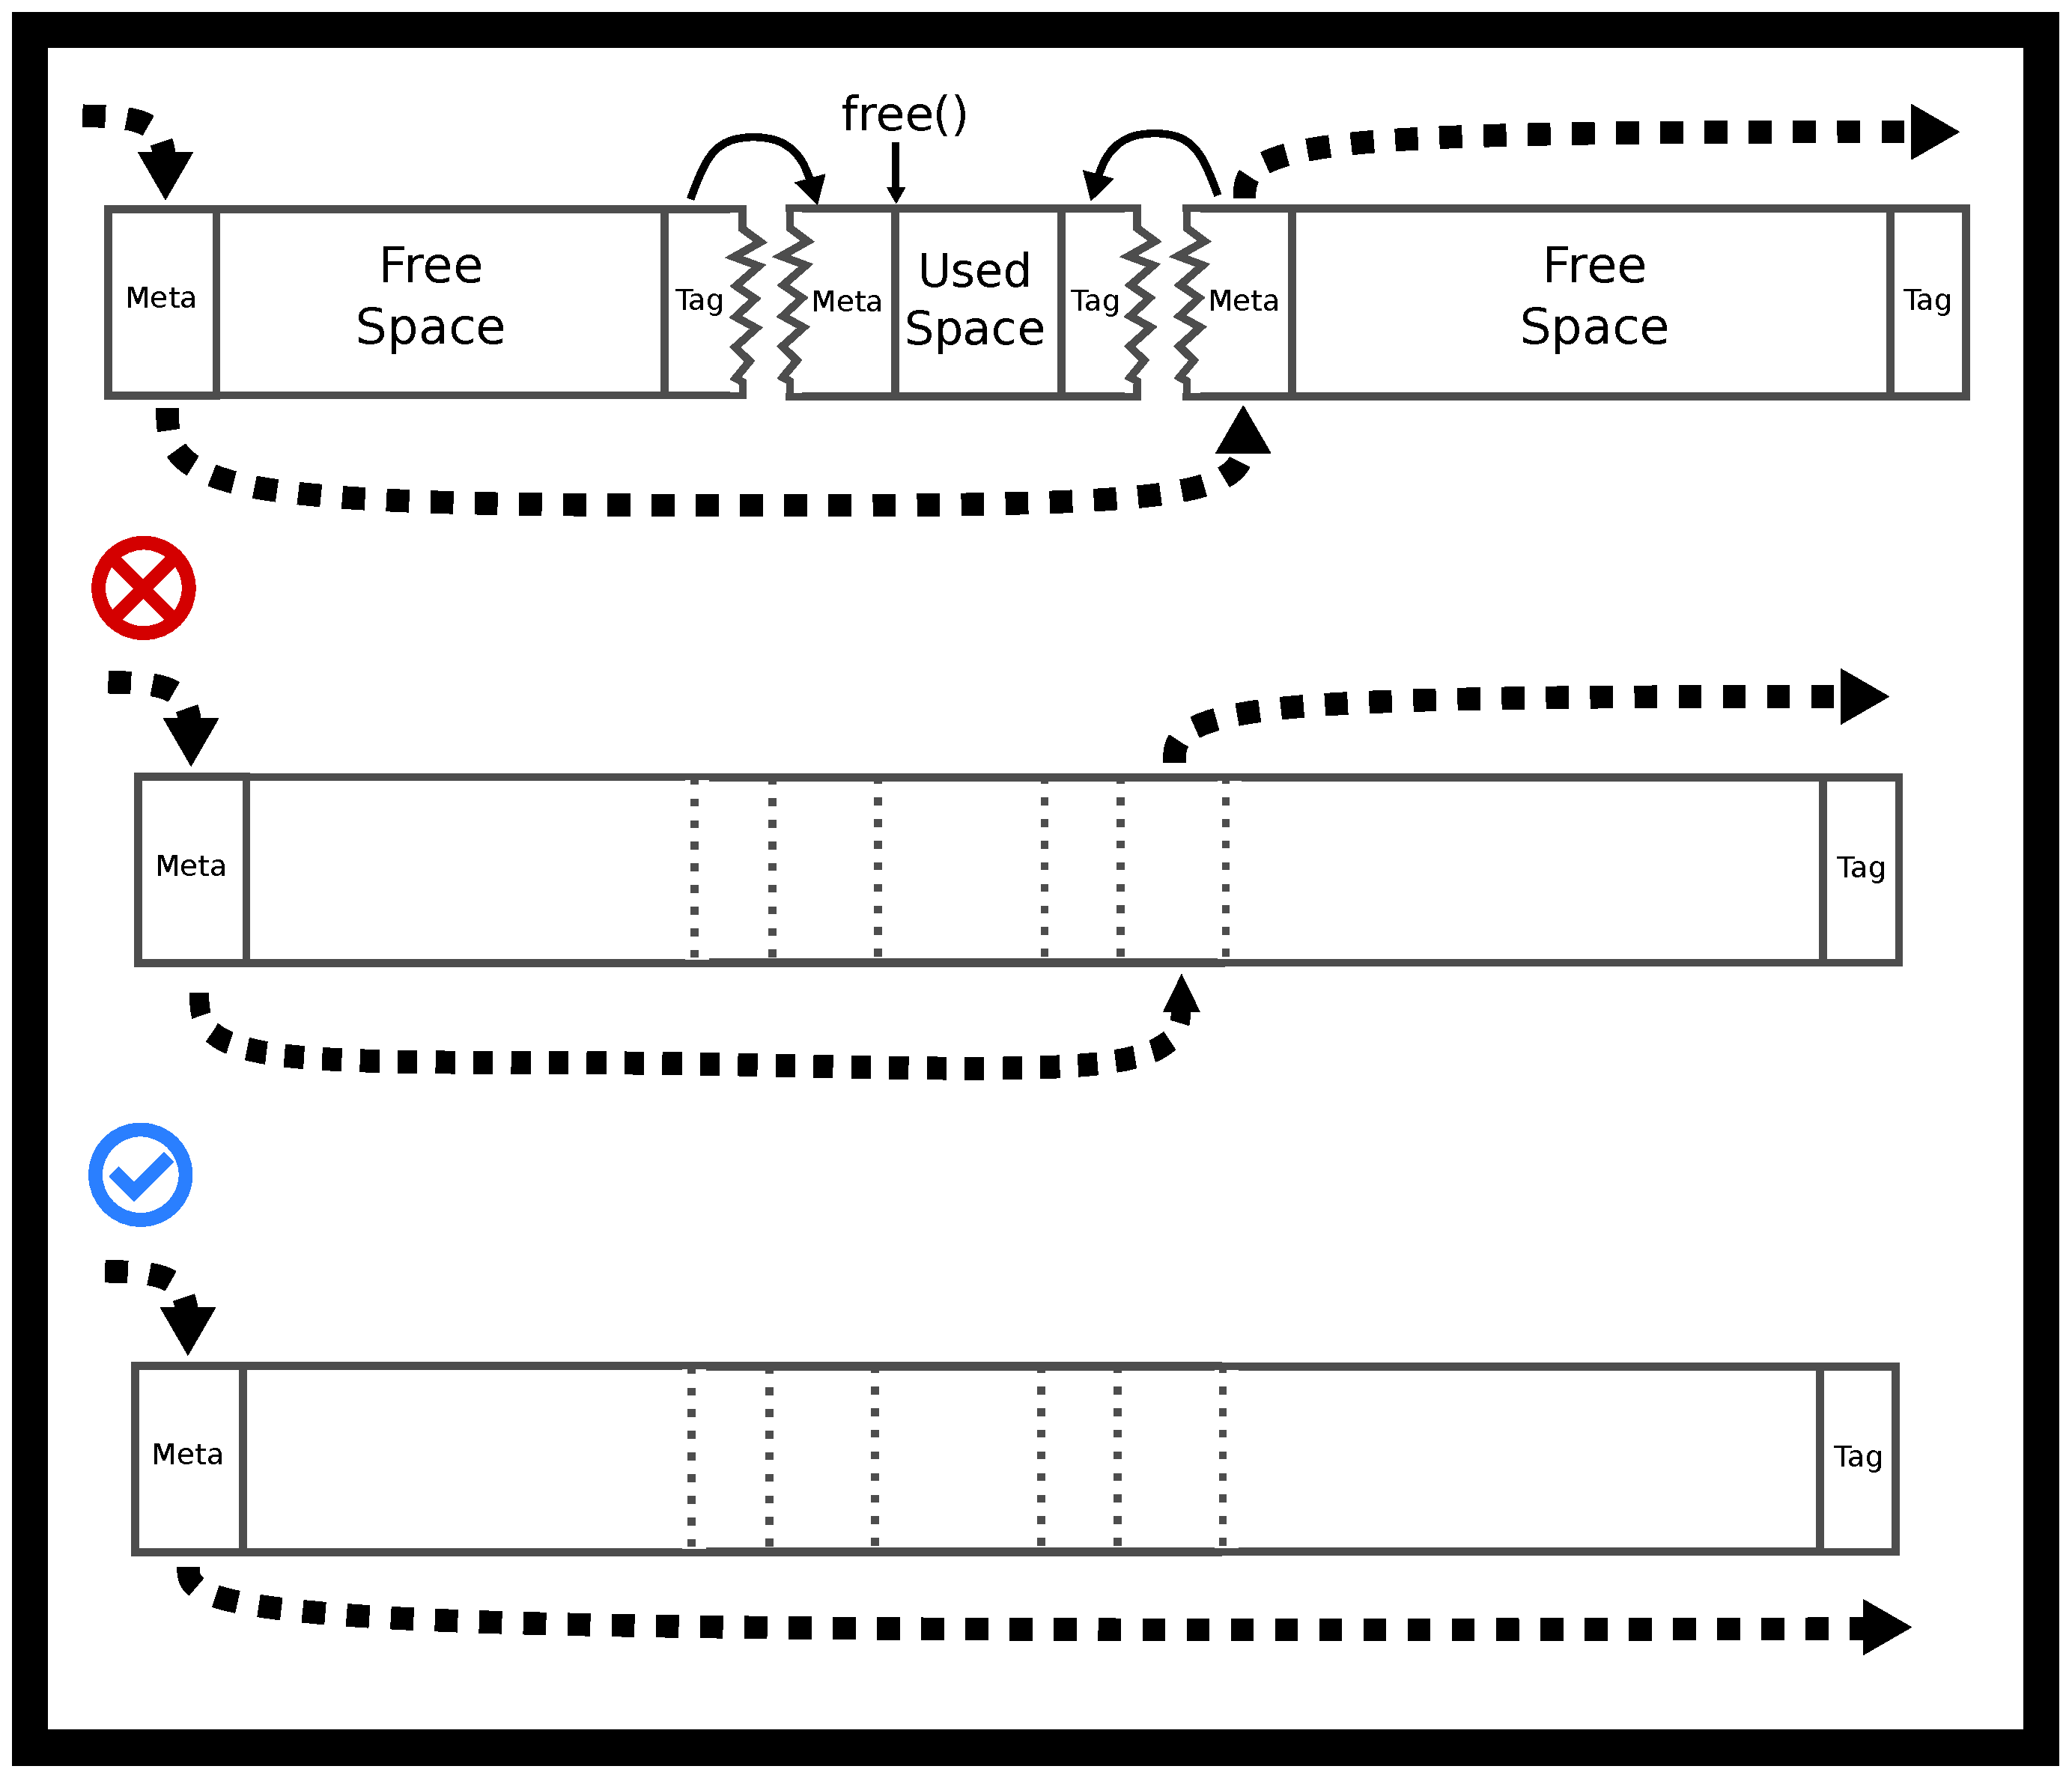
\includegraphics[width=.7\textwidth]{malloc/drawings/free_list_ptrs.eps}
\caption{Free list good and bad coalesce}
\end{figure}

We recommend when trying to implement malloc that you draw out all the cases conceptually and then write the code.

\subsubsection{Explicit linked list insertion policy}

The newly deallocated block can be inserted easily into two possible positions: at the beginning or in address order.
Inserting at the beginning creates a LIFO (last-in, first-out) policy.
The most recently deallocated spaces will be reused. Studies suggest fragmentation is worse than using address order \cite{10.1007/3-540-60368-9_19}.

Inserting in address order (``Address ordered policy'') inserts deallocated blocks so that the blocks are visited in increasing address order.
This policy required more time to free a block because the boundary tags (size data) must be used to find the next and previous unallocated blocks.
However, there is less fragmentation.

\section{Case study: Buddy Allocator, an example of a segregated list}

A segregated allocator is one that divides the heap into different areas that are handled by different sub-allocators dependent on the size of the allocation request.
Sizes are grouped into powers of two and each size is handled by a different sub-allocator and each size maintains its own free list.

A well known allocator of this type is the buddy allocator \cite[P. 85]{rangan1999foundations}.
We'll discuss the binary buddy allocator which splits allocation into blocks of size $2^n; n = 1, 2, 3, ...$ times some base unit number of bytes, but others also exist like Fibonacci split where the allocation is rounded up to the next Fibonacci number.
The basic concept is simple: If there are no free blocks of size $2^n$, go to the next level and steal that block and split it into two.
If two neighboring blocks of the same size become unallocated, they can be coalesced back together into a single large block of twice the size.

Buddy allocators are fast because the neighboring blocks to coalesce with can be calculated from the deallocated block's address, rather than traversing the size tags.
Ultimate performance often requires a small amount of assembler code to use a specialized CPU instruction to find the lowest non-zero bit.

The main disadvantage of the Buddy allocator is that they suffer from \emph{internal fragmentation}, because allocations are rounded up to the nearest block size.
For example, a 68-byte allocation will require a 128-byte block.

\section{Further Reading}

There are many other allocation schemes.
One of three allocators used internally by the Linux Kernel.
See \href{http://man7.org/linux/man-pages/man3/malloc.3.html}{the man page} or the appendix of the book \ref{man_malloc}!

\begin{itemize}
\item
  \href{http://en.wikipedia.org/wiki/SLUB_\%28software\%29}{SLUB} (wikipedia)
\item
  \href{http://en.wikipedia.org/wiki/Buddy_memory_allocation}{Wikipedia's buddy memory allocation page}
\end{itemize}

\section{Topics}

\begin{itemize}
\item
  Best Fit
\item
  Worst Fit
\item
  First Fit
\item
  Buddy Allocator
\item
  Internal Fragmentation
\item
  External Fragmentation
\item
  sbrk
\item
  Natural Alignment
\item
  Boundary Tag
\item
  Coalescing
\item
  Splitting
\item
  Slab Allocation/Memory Pool
\end{itemize}

\section{Questions/Exercises}

\begin{itemize}
\tightlist
\item
  What is Internal Fragmentation? When does it become an issue?
\item
  What is External Fragmentation? When does it become an issue?
\item
  What is a Best Fit placement strategy? How is it with External Fragmentation? Time Complexity?
\item
  What is a Worst Fit placement strategy? Is it any better with External Fragmentation? Time Complexity?
\item
  What is the First Fit Placement strategy? It's a little bit better with Fragmentation, right? Expected Time Complexity?
\item
  Let's say that we are using a buddy allocator with a new slab of 64kb. How does it go about allocating 1.5kb?
\item
  When does the 5 line \keyword{sbrk} implementation of malloc have a use?
\item
  What is natural alignment?
\item
  What is Coalescing/Splitting? How do they increase/decrease fragmentation? When can you coalesce or split?
\item
  How do boundary tags work? How can they be used to coalesce or split?
\end{itemize}

\bibliographystyle{plainnat}
\bibliography{malloc/malloc}
